\documentclass[man,floatsintext]{apa6}
\usepackage{lmodern}
\usepackage{amssymb,amsmath}
\usepackage{ifxetex,ifluatex}
\usepackage{fixltx2e} % provides \textsubscript
\ifnum 0\ifxetex 1\fi\ifluatex 1\fi=0 % if pdftex
  \usepackage[T1]{fontenc}
  \usepackage[utf8]{inputenc}
\else % if luatex or xelatex
  \ifxetex
    \usepackage{mathspec}
  \else
    \usepackage{fontspec}
  \fi
  \defaultfontfeatures{Ligatures=TeX,Scale=MatchLowercase}
\fi
% use upquote if available, for straight quotes in verbatim environments
\IfFileExists{upquote.sty}{\usepackage{upquote}}{}
% use microtype if available
\IfFileExists{microtype.sty}{%
\usepackage{microtype}
\UseMicrotypeSet[protrusion]{basicmath} % disable protrusion for tt fonts
}{}
\usepackage{hyperref}
\hypersetup{unicode=true,
            pdftitle={Plant life history strategies predicted by satellite-detected drought},
            pdfauthor={J Grey Monroe, Brian Gill, \& Kathryn Turner},
            pdfkeywords={drought adaptation, life history evolution, remote sensing,
phylogeography, herbaria records},
            pdfborder={0 0 0},
            breaklinks=true}
\urlstyle{same}  % don't use monospace font for urls
\usepackage{graphicx,grffile}
\makeatletter
\def\maxwidth{\ifdim\Gin@nat@width>\linewidth\linewidth\else\Gin@nat@width\fi}
\def\maxheight{\ifdim\Gin@nat@height>\textheight\textheight\else\Gin@nat@height\fi}
\makeatother
% Scale images if necessary, so that they will not overflow the page
% margins by default, and it is still possible to overwrite the defaults
% using explicit options in \includegraphics[width, height, ...]{}
\setkeys{Gin}{width=\maxwidth,height=\maxheight,keepaspectratio}
\IfFileExists{parskip.sty}{%
\usepackage{parskip}
}{% else
\setlength{\parindent}{0pt}
\setlength{\parskip}{6pt plus 2pt minus 1pt}
}
\setlength{\emergencystretch}{3em}  % prevent overfull lines
\providecommand{\tightlist}{%
  \setlength{\itemsep}{0pt}\setlength{\parskip}{0pt}}
\setcounter{secnumdepth}{0}
% Redefines (sub)paragraphs to behave more like sections
\ifx\paragraph\undefined\else
\let\oldparagraph\paragraph
\renewcommand{\paragraph}[1]{\oldparagraph{#1}\mbox{}}
\fi
\ifx\subparagraph\undefined\else
\let\oldsubparagraph\subparagraph
\renewcommand{\subparagraph}[1]{\oldsubparagraph{#1}\mbox{}}
\fi

%%% Use protect on footnotes to avoid problems with footnotes in titles
\let\rmarkdownfootnote\footnote%
\def\footnote{\protect\rmarkdownfootnote}


  \title{Plant life history strategies predicted by satellite-detected drought}
    \author{J Grey Monroe\textsuperscript{1,2}, Brian Gill\textsuperscript{3}, \&
Kathryn Turner\textsuperscript{4}}
    \date{}
  
\shorttitle{Drought and life history}
\affiliation{
\vspace{0.5cm}
\textsuperscript{1} Graduate Degree Program in Ecology, Colorado State University, Fort Collins, CO\\\textsuperscript{2} College of Agriculture, Colorado State University, Fort Collins, CO\\\textsuperscript{3} Department of Ecology and Evolutionary Biology, Brown University, Provience, RI\\\textsuperscript{4} Biology Department, Pennsylvania State University, State College, PA}
\keywords{drought adaptation, life history evolution, remote sensing, phylogeography, herbaria records\newline\indent Word count: }
\usepackage{csquotes}
\usepackage{upgreek}
\captionsetup{font=singlespacing,justification=justified}

\usepackage{longtable}
\usepackage{lscape}
\usepackage{multirow}
\usepackage{tabularx}
\usepackage[flushleft]{threeparttable}
\usepackage{threeparttablex}

\newenvironment{lltable}{\begin{landscape}\begin{center}\begin{ThreePartTable}}{\end{ThreePartTable}\end{center}\end{landscape}}

\makeatletter
\newcommand\LastLTentrywidth{1em}
\newlength\longtablewidth
\setlength{\longtablewidth}{1in}
\newcommand{\getlongtablewidth}{\begingroup \ifcsname LT@\roman{LT@tables}\endcsname \global\longtablewidth=0pt \renewcommand{\LT@entry}[2]{\global\advance\longtablewidth by ##2\relax\gdef\LastLTentrywidth{##2}}\@nameuse{LT@\roman{LT@tables}} \fi \endgroup}


\usepackage{lineno}

\linenumbers

\authornote{

Correspondence concerning this article should be addressed to J Grey
Monroe, 307 University Ave, Fort Collins, CO 80523. E-mail:
\href{mailto:monroejg@colostate.edu}{\nolinkurl{monroejg@colostate.edu}}}

\abstract{
Identifying the environmental factors that predict the evolution of
annual and perennial life history strategies in plants is important for
understanding ecosystem functioning, perennial cropping systems, and is
a long-standing goal of evolutionary ecology. A classic hypothesis is
that annual and perennial strategies reflect adaptation to environments
that differ in relative drought frequency. We test this hypothesis in
Heliophila (Brassicaceae), a genus of flowering plants native to
Southern Africa using herbarium occurrence records and
satellite-detected drought histories. We find that perennial Heliophila
species are observed in environments where droughts are significantly
less frequent compared to annuals, especially with regards to summer
drought. These correlations remain predictive while controlling for
phylogeny, lending support to the hypothesis that drought associated
natural selection has shaped differences in the distributions of these
strategies. Additionally, the collection dates of herbarium records are
consistent with a scenario in which annual species escape drought prone
seasons. Together these results point to a model of evolution that
supports classical hypotheses favoring perenniality in environments that
experience less drought, compared to annuals which escape drought prone
seasons as seed. Thus, changing drought regimens during the Anthropocene
may threaten locally adapted species. 
}

\usepackage{amsthm}
\newtheorem{theorem}{Theorem}[section]
\newtheorem{lemma}{Lemma}[section]
\theoremstyle{definition}
\newtheorem{definition}{Definition}[section]
\newtheorem{corollary}{Corollary}[section]
\newtheorem{proposition}{Proposition}[section]
\theoremstyle{definition}
\newtheorem{example}{Example}[section]
\theoremstyle{definition}
\newtheorem{exercise}{Exercise}[section]
\theoremstyle{remark}
\newtheorem*{remark}{Remark}
\newtheorem*{solution}{Solution}
\begin{document}
\maketitle

\hypertarget{introduction}{%
\section{Introduction}\label{introduction}}

\hypertarget{life-history}{%
\subsection{Life history}\label{life-history}}

Plants exhibit extraordinary diversity in life history strategies, from
herbaceous species that complete the entire seed to seed life cycle in a
number of weeks \{Guo, 2012 \#73\} to trees that live for thousands of
years \{Brown 1996 \url{http://www.rmtrr.org/oldlist.htm} \}. Along this
continuum an important division exists, distinguishing annuals which
complete their seed to seed life cycle within a single calendar year
from perennials which can persist over multiple years and therefore
experience the entire range of seasonal conditions. The ecological
factors that explain the evolution of these alternative strategies
remains poorly resolved \{Friedman, 2015 \#523\}. Understanding the
drivers of selection for these alternative strategies is important
because annuals and perennials have differing impacts on ecosystem
functioning, such as higher nitrogen concentration in perennials and
larger specific root length in annuals that affect nutrient cycling
\{Garnier, 1997 \#280\}\{Roumet, 2006 \#738\}. Furthermore, predicting
the conditions that favor these strategies in nature is useful for
developing more sustainable perennial cropping systems \{Lelievre and
Volaire, 2009\}.

\hypertarget{hypotheses}{%
\subsection{Hypotheses}\label{hypotheses}}

Seasonal drought conditions can represent a severe challenge to the
persistence of individual organisms. Well-established hypotheses suggest
that an annual life history is adaptive in environments where frequent
droughts makes an escape from stressful drought conditions in the form
of seed advantageous \{Stearns 1992\}\{Silvertown and Charlesworth,
2001\}. These hypotheses are based on models of life history evolution
in which short life cycles are favored in unpredictable environments or
those with frequent stressful conditions. Plants are expected to be more
likely to survive a drought that cooccurs with the seed phase of a
plant's life cycle in which they are most resistant to desiccation.
Previous efforts to address this hypothesis have yielded mixed or
qualitative results. Transitions to annuality in Oenothera were
associated with warmer summers and drier winters, but not with increased
drought directly \{Evans, 2005 \#260\}. Annual and perennial species of
Nemesia were qualitatively associated with winter rather and summer
rainfall environments respectively \{Datson, 2008\}. Similarly, annual
species of Scorzoneroides were associated with environments classified
as \enquote{unpredictable} \{Cruz-Mazo, 2009 \#598\}. Annual and
perennial varieties of the wild rice species Oryza rufipogon were
observed more frequently in dry and humid climates, respectively
\{Morishima et al.~1984\}. While these reports suggest the prominence of
annuals in environments considered more arid, a quantitative assessment
of how historic drought frequency may favor annual or perennial life
history strategies remains lacking.

\hypertarget{summary}{%
\subsection{Summary}\label{summary}}

Here we combine a long-term dataset of global imaging with metadata from
natural history collections to test classic hypotheses about the
evolution of life history strategies within the African endemic mustard
genus, Heliophila L. (Brassicaceae). If annual species temporally escape
drought as seed, then drought frequency should be an important
determinant of the distribution of life history strategies across the
landscape, and annual species should be more commonly associated with
drought prone regions than perennial species. Furthermore, if annual
species have adapted to escape drought prone seasons as seeds,
observations of annual species should be rare during drought prone
seasons. Phylogenetic relatedness can have significant non-random
effects on species distributions and life history traits (cite), and
therefore we assessed the relationship between life history distribution
and drought frequency in a phylogenetically controlled background.

\hypertarget{methods}{%
\section{Methods}\label{methods}}

\hypertarget{data}{%
\subsection{Data}\label{data}}

\hypertarget{drought}{%
\subsubsection{Drought}\label{drought}}

Remotely sensed data is a valuable tool for characterizing seasonal
patterns in drought \{AghaKouchak 2015\}. With these data, we can
exploit the fact that satellite imagery can detect reductions in plant
cover and moisture at landscape scales that are characteristic of
drought conditions. Unlike weather station data, which is limited in
geographic coverage, and manual observation, which is limited in scope,
satellite detected data provides a long term global historical record of
drought events at fine temporal and spatial resolutions. One such
measure, the Vegetative Health Index (VHI), has been collected since
1981 by NOAA AVHRR satellites and is a combined measure of thermal and
vegetative parameters. VHI quantifies drought induced vegetative stress
weekly by detecting reduced plant cover based on the normalized
difference vegetation index (Vegetative Condition Index) combined with
reductions in moisture associated with anomalies in thermal spectra
(Temperature Condition Index). Put most simply, the VHI detects drought
by identifying environments that appear unusually brown and dry for that
location and time of the year.

This data provides a global, long term, and quantitative perspective on
drought variability. The VHI database (see methods) presents a valuable
resource to study seasonal patterns in the frequency of drought across
environments and to test hypotheses about the effect of drought on
ecological and evolutionary processes. As such, it has been validated as
a tool for detecting drought and predicting crop yields \{Kogan 1997\}.
It has also proven useful for predicting infraspecific variation in
drought tolerance traits and genes \{Mojica et al 2016\}\{Dittberner et
al 2018\}\{Monroe et al 2018\}.

VHI quantifies drought induced vegetative stress weekly by detecting
reduced plant cover based on the normalized difference vegetation index
(Vegetative Condition Index) combined with reductions in moisture
associated with anomalies in thermal spectra (Temperature Condition
Index). Put most simply, the VHI detects drought by identifying
environments that appear unusually brown and dry for that location and
time of the year.

The Vegetative Health Index (VHI) was used to examine seasonal drought
frequency at the collection locations of Heliophila herbarium specimens.
The VHI is a satellite-detected drought measurement method based on
observations of vegetative stress caused by drought \{Kogan, 1995
\#534\}, combining deviations from historic climatic (Temperature
Condition Index) and vegetative conditions (Vegetative Condition Index).
The VHI has been measured weekly at 16km2 spatial resolution since XXXX.
The frequencies of observing drought conditions (VHI\textless{}40,
standard recommended by NOAA developers of VHI) during the southern
hemisphere spring (quarter surrounding spring equinox), summer (quarter
surrounding summer solstice), fall (quarter surrounding fall equinox),
and winter (quarter surrounding winter solstice) were calculated
globally from 1981 to 2015. These values were calculated for the
collection location of each Heliophila herbarium specimen in our
filtered dataset.

NDVI = (Ch2 - Chl)/(Ch2 + Chl)

\[NDVI = \frac{NIR - Red}{NIR + Red}\]

\[VCI = 100\frac{NDVI - NDVI_{min}}{NDVI_{max} - NDVI_{min}}\]

\[TCI = 100\frac{T - T{min}}{T{max} - T{min}}\]

\[VHI = 0.5(VCI) + 0.5(TCI)\] This data provides a global, long term,
and quantitative perspective on drought variability. The VHI database
presents a valuable resource to study seasonal patterns in the frequency
of drought across environments and to test hypotheses about the effect
of drought on ecological and evolutionary processes. As such, it has
been validated as a tool for detecting drought and predicting crop
yields ({\textbf{???}}). It has also proven useful for predicting
infraspecific variation in drought tolerance traits and genes
(Dittberner et al., 2018; Mojica et al., 2016; Monroe et al., 2018).

\hypertarget{life-history-1}{%
\subsubsection{Life history}\label{life-history-1}}

Heliophila is a genus of flowering plants endemic to the southern
portion of Africa including the Cape Floristic and Succulent Karoo
Regions which are among the most botanically diverse environments on
Earth. Indeed, the estimated \textasciitilde{}50 Heliophila species are
considered to represent the most diverse genus of the family
Brassicaceae \{Mummenhoff, 2005 \#494\}. This genus includes both
perennial and annual species and this change in life history strategy
has likely arisen multiple independent times \{Appel \& Al-Shehbaz,
1997\}\{Mummenhoff, 2005 \#494\}. These multiple transitions between
life history strategy and it's well documented record in global herbaria
provided the ideal system to address classic hypotheses about the
evolutionary drivers of annual and perennial life history strategies.

\hypertarget{phyologeny}{%
\subsubsection{Phyologeny}\label{phyologeny}}

Herbaria records and satellite detected drought provide data with which
the distributions of annual and perennial species can be compared with
respect to historic drought frequency. However, it is necessary to
control for the demographic history caused by common ancestry of species
if evolutionary processes such as natural selection are to be invoked as
explanations for any differences observed. If, for example, annual and
perennial species show significantly different ranges with respect to
historic drought this could be confounded by common ancestry if annuals
originated from a common ancestor and vice versa. In this case, it would
be challenging to distinguish between natural selection and demographic
history. On the other hand, if annual and perennial life history
strategies arose independently in multiple species, controlling for
phylogenetic relationships allows us to better account for demography
and make stronger assertions about the importance of processes such as
natural selection to explain patterns.

Heliophila is a charismatic genus of flowering plants from the
Brassicaceae provides a valuable model to study the evolution of annual
and perennial life history strategies because each has arisen
independently multiple times within the genus. These independent origins
allow for phylogenetically constrained analyses comparing the climate
distributions of annual and perennial species, to gain greater insight
into the role of selection.

Aligned Heliophila ITS sequences were obtained from previous work by
Mandáková et al.~\{Mandáková, 2012 \#339\}. Aethionema, Alliaria,
Cardamine, Chamira, and Rorippa ITS records from were downloaded from
Genbank (link) and aligned together with Heliophila ITS sequences using
MAFFT as outgroups? (cite). Model selection for construction of
phylogeny was performed in jModeltest2 with CIPRES (cite). Based on this
analysis, \(GTR + L\) were selected. Ultrametric phylogeny was estimated
with branch lengths as relative time (details). Life history character
states were used based on habit reported by Mummemhoff et
al.~\{Mummenhoff, 2005 \#494\}. Species reported to have any form of
perennial life history (such as biennial\ldots{}) were classified for
analyses here as perennial, where species reported to have strictly
annual life histories were classified for analyses here as annual.

\hypertarget{herbarium-specimens}{%
\subsubsection{Herbarium Specimens}\label{herbarium-specimens}}

Botanists have collected and maintained over 350 million botanical
specimens worldwide over the past 300 years (Lang et al 2018). These
collections, housed in herbaria, comprise an enormous, yet largely
untapped, ecological dataset. These specimens are increasingly being
recognized as an invaluable and underutilized source of data pertaining
to biological responses to past environmental conditions (Pyke et
al.~2010). Herbarium specimens and their associated metadata have been
used since the 1960s to study species' geographical distributions
(reviewed in Lang et al.~2018). Herbarium specimens have been used to
track plant responses to climate change using herbarium time-series,
including the relationships between traits, geography, and climate.
\{Wolf et al.~2016, Davis et al.~2015, Stropp et al.~2017\}. A
potentially fruitful approach combines herbarium data with remotely
sensed data sets that characterize the environmental and climatic
conditions across landscapes. For example, remotely sensed global
ultraviolet-B radiation exposure may explain differences in trichome
phenotypes, observed from herbarium specimens, between the native and
invasive ranges of two herbaceous plants (Václavík et al.~2017).

Herbarium specimen records for all Heliophila species were downloaded
from the Global Biodiversity Information Facility (gbif.org) on July 21,
2018. Several filtering steps were employed to clean this data (see Sup
Mat. R code). For these analyses, records were restricted to those which
are associated with a physical herbarium specimen, rather than other
types of observations. Consequentially, this sample represents
individuals in a narrow range of vegetative and/or flowering states --
for example, herbarium specimens cannot be collected for individuals
existing as seed. Analyses were restricted to Heliophila species with
previously-reported life history information \{Mummenhoff, 2005 \#494\};
42 of \textasciitilde{}50 named species in this genus were used. Only
records including geo-referenced information (latitude and longitude of
collection site) were used for downstream analyses of historic drought
frequency. To discard records likely to be erroneous and to restrict
analyses to plants in their native, non-cultivated, habitats, records
occurring outside of the native range (roughly, the southern half of
Africa) were removed. This excluded specimens such as those growing in
likely cultivation in Australia or terrestrial plants recorded from
non-terrestrial oceanic locations.. Finally, duplicate records, based on
species, collection location coordinates, and date, were removed.

We downloaded 8670 records from GBIF.

\hypertarget{analyses}{%
\subsection{Analyses}\label{analyses}}

\hypertarget{drought-frequency}{%
\subsubsection{Drought frequency}\label{drought-frequency}}

\hypertarget{herbarium-clean-up}{%
\subsubsection{Herbarium clean up}\label{herbarium-clean-up}}

We filtered raw GBIF by restricting our analyses to

\begin{itemize}
\tightlist
\item
  Species with reported life history\\
\item
  Records with geospatial data\\
\item
  Records from collection sites classified as land pixels
\item
  Records for perserved specimens
\item
  Records from Africa
\item
  Non-duplicate records (ie. identical species, location, collection
  date)
\end{itemize}

\hypertarget{phylogeny}{%
\subsubsection{Phylogeny}\label{phylogeny}}

\hypertarget{contrast}{%
\subsubsection{Contrast}\label{contrast}}

To evaluate the hypothesis that annual and perennial life history
strategies reflect adaptations to alternative drought regimes, we tested
the corresponding prediction that the observed distributions of annual
and perennial Heliophila species would be significantly associated with
historic drought frequency. To do so, the average drought frequency for
each season was calculated across the herbarium specimen collection
locations for each species. The relationship between drought frequencies
across each taxon's range and life habitat (annual or perennial) was
evaluated using Firth's penalized-likelihood logistic regression and
phylogenetic logistic regression.

\hypertarget{collection-dates}{%
\subsubsection{Collection dates}\label{collection-dates}}

To test the hypothesis that annual species have adapted to escape
drought prone seasons as seeds, collection dates for herbarium specimens
were compared between annual and perennial species. Comparisons of
distributions were made by Two-sample Kolmogorov-Smirnov test, t-test,
and Barlett variance test using R (supplemental script 2) \{cite R\}.
\#\#\# Software We used R (Version 3.5.1; R Core Team, 2018) and the
R-packages \emph{ape} (Version 5.2; Paradis \& Schliep, 2018; Orme et
al., 2018; Soetaert, 2018), \emph{bindrcpp} (Version 0.2.2; Müller,
2018), \emph{caper} (Version 1.0.1; Orme et al., 2018), \emph{coda}
(Version 0.19.2; Plummer, Best, Cowles, \& Vines, 2006), \emph{diagram}
(Version 1.6.4; Soetaert, 2017), \emph{dplyr} (Version 0.7.8; Wickham et
al., 2018), \emph{forcats} (Version 0.3.0; Wickham, 2018a), \emph{gee}
(Version 4.13.19; R by Thomas Lumley \& author., 2015), \emph{geiger}
(Version 2.0.6; Alfaro et al., 2009; Eastman, Alfaro, Joyce, Hipp, \&
Harmon, 2011; Harmon, Weir, Brock, Glor, \& Challenger, 2008; Slater et
al., 2012), \emph{ggplot2} (Version 3.1.0; Wickham, 2016),
\emph{logistf} (Version 1.23; Heinze \& Ploner, 2018), \emph{maps}
(Version 3.3.0; Richard A. Becker, Ray Brownrigg. Enhancements by Thomas
P Minka, \& Deckmyn., 2018), \emph{MASS} (Version 7.3.51.1; Venables \&
Ripley, 2002), \emph{Matrix} (Version 1.2.15; Bates \& Maechler, 2018),
\emph{MCMCglmm} (Version 2.26; Hadfield, 2010), \emph{mvtnorm} (Version
1.0.8; Genz \& Bretz, 2009), \emph{papaja} (Version 0.1.0.9842; Aust \&
Barth, 2018), \emph{phylolm} (Version 2.6; Ho \& Ane, 2014),
\emph{phytools} (Version 0.6.60; Revell, 2012), \emph{purrr} (Version
0.2.5; Henry \& Wickham, 2018), \emph{raster} (Version 2.8.4; Hijmans,
2018), \emph{readr} (Version 1.2.1; Wickham et al., 2017), \emph{shape}
(Version 1.4.4; Soetaert, 2018), \emph{sp} (Version 1.3.1; Pebesma \&
Bivand, 2005), \emph{stringr} (Version 1.3.1; Wickham, 2018b),
\emph{tibble} (Version 1.4.2; Müller \& Wickham, 2018), \emph{tidyr}
(Version 0.8.2; Wickham \& Henry, 2018), and \emph{tidyverse} (Version
1.2.1; Wickham, 2017) for all our analyses.

\hypertarget{results}{%
\section{Results}\label{results}}

To test the hypothesis that annual and perennial plants reflect
adaptation to alternative drought environments we examined the landscape
distribution of life history strategies in the large and diverse mustard
genus, \emph{Heliophila} Figure \ref{fig:phylogeny}. Using both
herbarium specimen metadata and a 30 year dataset of satellite generated
climate information, we tested the prediction that annual species are
more often observed in drought-prone locations than perennial species,
when controlling for phylogenetic relatedness. We found that drought
frequency is significantly different between the distributions of annual
and perennial species, with annuals being found in environments with
significantly more frequent drought, and that this signal is strongest
during the summer. These results remain significant while controlling
for the phylogenetic relationships of Heliophila species, yielding
support for the role that natural selection has played in driving
contemporary distributions of these alternatives strategies in relation
to drought regimes.



\begin{figure}[!h]
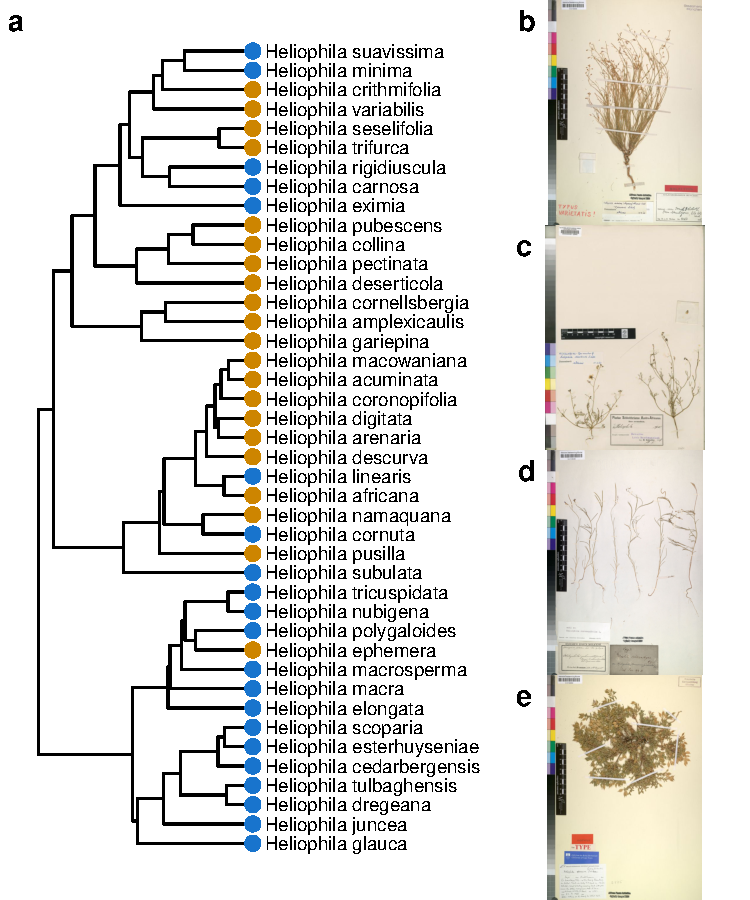
\includegraphics[width=\textwidth]{../figures/phylogeny} \caption{Phylogeny of Heliophila.}\label{fig:phylogeny}
\end{figure}

\hypertarget{gbif-records}{%
\subsubsection{GBIF records}\label{gbif-records}}

Out of 8670 \emph{Heliophila} GBIF recrods, 6634 were for species with
reported life history (Mummenhoff, Al-Shehbaz, Bakker, Linder, \&
Mühlhausen, 2005), 3653 had geospatial data, 3460 were located on pixels
classified as land having drought measurements, 3457 were located in
Africa, 3162 were not duplicated. After all filtering steps, 2192
records for 42 species (Figure \ref{tab:gbifrecordsmap}, Table
\ref{tab:speciesmeanstable}) passed.




\begin{figure}
\centering
\includegraphics{../figures/gbifrecords.pdf}
\caption{\label{fig:gbifrecordsmap}Map of 2192 GBIF records that passed quality
filtering.}
\end{figure}

\begin{center}
\begin{ThreePartTable}
\begin{TableNotes}[para]
\normalsize{\textit{Note.} LH = Life history (a = annual, p = perennial). n=sample size of GBIF records. Seasons are mean drought frequencies observed at locations of records.}
\end{TableNotes}
\small{
\begin{longtable}{lllllll}\noalign{\getlongtablewidth\global\LTcapwidth=\longtablewidth}
\caption{\label{tab:speciesmeanstable}Heliophila species records and the mean drought frequencies during different seasons at the location of records }\\
\toprule
Species & \multicolumn{1}{c}{LH} & \multicolumn{1}{c}{n} & \multicolumn{1}{c}{Winter} & \multicolumn{1}{c}{Spring} & \multicolumn{1}{c}{Summer} & \multicolumn{1}{c}{Fall}\\
\midrule
Heliophila acuminata & a & 28 & 0.32 & 0.38 & 0.41 & 0.36\\
Heliophila africana & a & 91 & 0.33 & 0.35 & 0.34 & 0.34\\
Heliophila amplexicaulis & a & 60 & 0.32 & 0.36 & 0.39 & 0.33\\
Heliophila arenaria & a & 65 & 0.34 & 0.37 & 0.38 & 0.34\\
Heliophila carnosa & p & 129 & 0.33 & 0.37 & 0.39 & 0.31\\
Heliophila cedarbergensis & p & 3 & 0.40 & 0.43 & 0.32 & 0.27\\
Heliophila collina & a & 16 & 0.35 & 0.47 & 0.48 & 0.45\\
Heliophila cornellsbergia & a & 2 & 0.33 & 0.42 & 0.35 & 0.21\\
Heliophila cornuta & p & 101 & 0.35 & 0.40 & 0.40 & 0.34\\
Heliophila coronopifolia & a & 40 & 0.37 & 0.42 & 0.40 & 0.37\\
Heliophila crithmifolia & a & 97 & 0.35 & 0.42 & 0.45 & 0.38\\
Heliophila descurva & a & 12 & 0.36 & 0.38 & 0.38 & 0.29\\
Heliophila deserticola & a & 133 & 0.48 & 0.48 & 0.46 & 0.45\\
Heliophila digitata & a & 30 & 0.33 & 0.38 & 0.44 & 0.38\\
Heliophila dregeana & p & 17 & 0.33 & 0.37 & 0.33 & 0.32\\
Heliophila elongata & p & 82 & 0.26 & 0.32 & 0.30 & 0.25\\
Heliophila ephemera & a & 3 & 0.14 & 0.27 & 0.31 & 0.26\\
Heliophila esterhuyseniae & p & 3 & 0.21 & 0.30 & 0.37 & 0.27\\
Heliophila eximia & p & 12 & 0.42 & 0.41 & 0.32 & 0.34\\
Heliophila gariepina & a & 12 & 0.50 & 0.53 & 0.48 & 0.41\\
Heliophila glauca & p & 35 & 0.29 & 0.35 & 0.34 & 0.33\\
Heliophila juncea & p & 150 & 0.32 & 0.37 & 0.39 & 0.35\\
Heliophila linearis & p & 94 & 0.32 & 0.33 & 0.28 & 0.30\\
Heliophila macowaniana & a & 31 & 0.33 & 0.38 & 0.44 & 0.39\\
Heliophila macra & p & 22 & 0.30 & 0.30 & 0.32 & 0.29\\
Heliophila macrosperma & p & 5 & 0.28 & 0.36 & 0.35 & 0.25\\
Heliophila minima & p & 35 & 0.36 & 0.45 & 0.51 & 0.39\\
Heliophila namaquana & a & 16 & 0.39 & 0.46 & 0.48 & 0.39\\
Heliophila nubigena & p & 19 & 0.31 & 0.36 & 0.43 & 0.38\\
Heliophila pectinata & a & 16 & 0.27 & 0.34 & 0.50 & 0.34\\
Heliophila polygaloides & p & 12 & 0.40 & 0.48 & 0.42 & 0.34\\
Heliophila pubescens & a & 9 & 0.31 & 0.40 & 0.48 & 0.39\\
Heliophila pusilla & a & 45 & 0.32 & 0.38 & 0.38 & 0.34\\
Heliophila rigidiuscula & p & 201 & 0.30 & 0.33 & 0.28 & 0.24\\
Heliophila scoparia & p & 106 & 0.31 & 0.37 & 0.36 & 0.31\\
Heliophila seselifolia & a & 80 & 0.36 & 0.42 & 0.45 & 0.40\\
Heliophila suavissima & p & 92 & 0.30 & 0.39 & 0.42 & 0.31\\
Heliophila subulata & p & 103 & 0.29 & 0.33 & 0.31 & 0.29\\
Heliophila tricuspidata & p & 8 & 0.28 & 0.33 & 0.38 & 0.30\\
Heliophila trifurca & a & 77 & 0.45 & 0.48 & 0.48 & 0.43\\
Heliophila tulbaghensis & p & 3 & 0.36 & 0.41 & 0.36 & 0.35\\
Heliophila variabilis & a & 97 & 0.35 & 0.41 & 0.40 & 0.37\\
\bottomrule
\addlinespace
\insertTableNotes
\end{longtable}
}
\end{ThreePartTable}
\end{center}

\hypertarget{drought-frequency.}{%
\subsubsection{Drought frequency.}\label{drought-frequency.}}




\begin{figure}
\centering
\includegraphics{../figures/life_history_drought_boxplots.pdf}
\caption{\label{fig:boxplots}Comparison of drought frequency across seasons measured
at the GBIF records of annual and perennial species of Heliophila.}
\end{figure}

\begin{table}[tbp]
\begin{center}
\begin{threeparttable}
\caption{\label{tab:firthmodelstable}Logistic regressions between life history, and the mean drought frequency observed at herbaria collection sites of Heliophila species. }
\begin{tabular}{lll}
\toprule
Predictor & \multicolumn{1}{c}{Estimate} & \multicolumn{1}{c}{p.value}\\
\midrule
Intercept & 2.2575 & 0.1739\\
Winter drought freq. & -6.7484 & 0.1661\\ \midrule
Intercept & 4.5594 & 0.0443\\
Spring drought freq. & -11.7895 & 0.0423\\ \midrule
Intercept & 7.1742 & 0.0011\\
Summer drought freq. & -18.2999 & 0.0010\\ \midrule
Intercept & 6.4226 & 0.0029\\
Fall drought freq. & -19.0512 & 0.0026\\ \midrule
\bottomrule
\addlinespace
\end{tabular}
\begin{tablenotes}[para]
\normalsize{\textit{Note.} Firth's penalized logistic regression. Annual species were scored as 0 and perennial species as 1.}
\end{tablenotes}
\end{threeparttable}
\end{center}
\end{table}

\begin{table}[tbp]
\begin{center}
\begin{threeparttable}
\caption{\label{tab:phylomodelstable}Phlyogenetically constrained logistic regressions between life history, and the mean drought frequency observed at herbaria collection sites of Heliophila species. }
\begin{tabular}{lll}
\toprule
Predictor & \multicolumn{1}{c}{Estimate} & \multicolumn{1}{c}{p.value}\\
\midrule
Intercept & 0.7231 & 0.6636\\
Winter drought freq. & -1.5452 & 0.7274\\ \midrule
Intercept & 5.0107 & 0.0534\\
Spring drought freq. & -12.9014 & 0.0464\\ \midrule
Intercept & 7.7093 & 0.0054\\
Summer drought freq. & -19.9056 & 0.0042\\ \midrule
Intercept & 7.0162 & 0.0082\\
Fall drought freq. & -20.8174 & 0.0067\\ \midrule
\bottomrule
\addlinespace
\end{tabular}
\begin{tablenotes}[para]
\normalsize{\textit{Note.} Annual species were scored as 0 and perennial species as 1.}
\end{tablenotes}
\end{threeparttable}
\end{center}
\end{table}





\begin{figure}
\centering
\includegraphics{../figures/life_history_drought_means_line.pdf}
\caption{\label{fig:lineplots}Comparison (mean +- SE) of drought frequency across
seasons measured at the GBIF records of annual and perennial species of
Heliophila.}
\end{figure}

\hypertarget{collection-dates-1}{%
\subsubsection{Collection dates}\label{collection-dates-1}}




\begin{figure}
\centering
\includegraphics{../figures/collection_dates.pdf}
\caption{\label{fig:collectiondates}Collection dates of GBIF records of annual and
perennial species of Heliophila.}
\end{figure}

\hypertarget{discussion}{%
\section{Discussion}\label{discussion}}

\hypertarget{summary-1}{%
\subsection{Summary}\label{summary-1}}

We found that the distribution of annual and perennial species of
Heliophila is significantly predicted by satellite detected historic
drought frequencies. Annual species are found in environments that
experience more frequent drought during the summer and fall quarters
compared to perennials. This relationship was consistent while
controlling for phylogenetic relatedness among the taxa studied,
indicating that these distributions cannot be explained entirely by
common ancestry., These results support the hypothesis that natural
selection has played a role in shaping the contemporary distributions of
these alternative life-history strategies.

\hypertarget{relationship-to-previous-hypotheseswork}{%
\subsection{Relationship to previous
hypotheses/work}\label{relationship-to-previous-hypotheseswork}}

These findings support classical theoretical predictions about the
adaptive value of annual and perennial life history strategies. Taken
together, they suggest that in Heliophila, annual species are adapted to
environments with increased summer droughts by avoiding these seasons in
a dormant seed phase of their life cycle. Indeed, we found that very few
annuals are collected during this season, supporting the prediction that
they are not in a vegetative and/or reproductive phase at this time.
Traditionally, the focus has been on the evolutionary origins of annual
life histories \{citations\}. However, we also find evidence that the
transition to perenniality could be explained by historical drought
regimes. The phylogeny reveals several transitions from annual to
perennial life history. Perennials may be able to out complete annual
relatives in environments where the infrequency of drought favors
strategies that allow plants to benefit from growth over many seasons.

\hypertarget{caveats}{%
\subsection{Caveats}\label{caveats}}

Correlation does not prove causation. But it does indicate predictive
power and is consistent with adaptive hypotheses. Herbarium collections
and their associated data do not represent systematic or random sampling
of a species distribution. Significant biases in collecting exist, which
we have not necessarily controlled for here, and may have some effect on
our findings, such as a bias toward collecting near roads or near the
locations of natural history collections (Daru et al.~2018, Heberling,
in press). Despite these biases, the Cape Floristic region is a
biodiversity hotspot and one of the most botanically well sampled
regions on Earth (Daru et al.~2018, Heberling, in press?), suggesting
that this may currently be the optimal region for our analyses of life
history distribution. Future research will benefit from systematic
sampling efforts to avoid these noted biases. The climate data used here
are assessed only from 198X-XXXX and do not reflect conditions at the
estimated divergence dates of these species (XXX million of years ago).
Rather, the results suggest that the current distributions of annual and
perennial species reflect a history of environmental filtration and
ongoing natural selection. That is, their distributions are non-random
with respect to historic drought and this is not explained by phylogeny.

\hypertarget{broader-implications}{%
\subsection{Broader implications}\label{broader-implications}}

These findings suggest that rapidly changing drought regimes threaten
species adapted to current environments. Studies predict changing
drought regimes. This could have impacts on ecosystem functioning. This
should also be considered when thinking about using perennial crops.
Studies predict changing drought regimes.

\hypertarget{conclusions}{%
\subsection{Conclusions}\label{conclusions}}

Perenniality appears to be adaptive in environments with less frequent
drought. This work demonstrates the power of emerging data to address
outstanding classic hypotheses in ecology and evolution.

\hypertarget{acknowledgments}{%
\section{Acknowledgments}\label{acknowledgments}}

This work was supported by NSF no. USDA grant no. XXX to J.G.M.

\hypertarget{references}{%
\section{References}\label{references}}

\newpage

\begingroup
\setlength{\parindent}{-0.5in}
\setlength{\leftskip}{0.5in}

\hypertarget{refs}{}
\leavevmode\hypertarget{ref-R-geiger_a}{}%
Alfaro, M., Santini, F., Brock, C., Alamillo, H., Dornburg, A., Rabosky,
D., \ldots{} Harmon, L. (2009). Nine exceptional radiations plus high
turnover explain species diversity in jawed vertebrates.
\emph{Proceedings of the National Academy of Sciences of the United
States of America}, \emph{106}, 13410--13414.

\leavevmode\hypertarget{ref-R-papaja}{}%
Aust, F., \& Barth, M. (2018). \emph{papaja: Create APA manuscripts with
R Markdown}. Retrieved from \url{https://github.com/crsh/papaja}

\leavevmode\hypertarget{ref-R-Matrix}{}%
Bates, D., \& Maechler, M. (2018). \emph{Matrix: Sparse and dense matrix
classes and methods}. Retrieved from
\url{https://CRAN.R-project.org/package=Matrix}

\leavevmode\hypertarget{ref-dittberner2018natural}{}%
Dittberner, H., Korte, A., Mettler-Altmann, T., Weber, A., Monroe, G.,
\& Meaux, J. de. (2018). Natural variation in stomata size contributes
to the local adaptation of water-use efficiency in arabidopsis thaliana.
\emph{bioRxiv}, 253021.

\leavevmode\hypertarget{ref-R-geiger_b}{}%
Eastman, J., Alfaro, M., Joyce, P., Hipp, A., \& Harmon, L. (2011). A
novel comparative method for identifying shifts in the rate of character
evolution on trees. \emph{Evolution}, \emph{65}, 3578--3589.

\leavevmode\hypertarget{ref-R-mvtnorm}{}%
Genz, A., \& Bretz, F. (2009). \emph{Computation of multivariate normal
and t probabilities}. Heidelberg: Springer-Verlag.

\leavevmode\hypertarget{ref-R-MCMCglmm}{}%
Hadfield, J. D. (2010). MCMC methods for multi-response generalized
linear mixed models: The MCMCglmm R package. \emph{Journal of
Statistical Software}, \emph{33}(2), 1--22. Retrieved from
\url{http://www.jstatsoft.org/v33/i02/}

\leavevmode\hypertarget{ref-R-geiger_d}{}%
Harmon, L., Weir, J., Brock, C., Glor, R., \& Challenger, W. (2008).
GEIGER: Investigating evolutionary radiations. \emph{Bioinformatics},
\emph{24}, 129--131.

\leavevmode\hypertarget{ref-R-logistf}{}%
Heinze, G., \& Ploner, M. (2018). \emph{Logistf: Firth's bias-reduced
logistic regression}. Retrieved from
\url{https://CRAN.R-project.org/package=logistf}

\leavevmode\hypertarget{ref-R-purrr}{}%
Henry, L., \& Wickham, H. (2018). \emph{Purrr: Functional programming
tools}. Retrieved from \url{https://CRAN.R-project.org/package=purrr}

\leavevmode\hypertarget{ref-R-raster}{}%
Hijmans, R. J. (2018). \emph{Raster: Geographic data analysis and
modeling}. Retrieved from
\url{https://CRAN.R-project.org/package=raster}

\leavevmode\hypertarget{ref-R-phylolm}{}%
Ho, L. S. T., \& Ane, C. (2014). A linear-time algorithm for gaussian
and non-gaussian trait evolution models. \emph{Systematic Biology},
\emph{63}, 397--408.

\leavevmode\hypertarget{ref-Mojica2016}{}%
Mojica, J. P., Mullen, J., Lovell, J. T., Monroe, J. G., Paul, J. R.,
Oakley, C. G., \& McKay, J. K. (2016). Genetics of water use physiology
in locally adapted Arabidopsis thaliana. \emph{Plant Science}.
doi:\href{https://doi.org/10.1016/j.plantsci.2016.03.015}{10.1016/j.plantsci.2016.03.015}

\leavevmode\hypertarget{ref-monroe2018drought}{}%
Monroe, J. G., Powell, T., Price, N., Mullen, J., Howard, A., Evans, K.,
\ldots{} McKay, J. (2018). Drought adaptation in nature by extensive
genetic loss-of-function. \emph{bioRxiv}, 372854.

\leavevmode\hypertarget{ref-mummenhoff2005phylogeny}{}%
Mummenhoff, K., Al-Shehbaz, I. A., Bakker, F. T., Linder, H. P., \&
Mühlhausen, A. (2005). Phylogeny, morphological evolution, and
speciation of endemic brassicaceae genera in the cape flora of southern
africa. \emph{Annals of the Missouri Botanical Garden}, 400--424.

\leavevmode\hypertarget{ref-R-bindrcpp}{}%
Müller, K. (2018). \emph{Bindrcpp: An 'rcpp' interface to active
bindings}. Retrieved from
\url{https://CRAN.R-project.org/package=bindrcpp}

\leavevmode\hypertarget{ref-R-tibble}{}%
Müller, K., \& Wickham, H. (2018). \emph{Tibble: Simple data frames}.
Retrieved from \url{https://CRAN.R-project.org/package=tibble}

\leavevmode\hypertarget{ref-R-caper}{}%
Orme, D., Freckleton, R., Thomas, G., Petzoldt, T., Fritz, S., Isaac,
N., \& Pearse, W. (2018). \emph{Caper: Comparative analyses of
phylogenetics and evolution in r}. Retrieved from
\url{https://CRAN.R-project.org/package=caper}

\leavevmode\hypertarget{ref-R-ape}{}%
Paradis, E., \& Schliep, K. (2018). Ape 5.0: An environment for modern
phylogenetics and evolutionary analyses in R. \emph{Bioinformatics},
\emph{xx}, xxx--xxx.

\leavevmode\hypertarget{ref-R-sp}{}%
Pebesma, E. J., \& Bivand, R. S. (2005). Classes and methods for spatial
data in R. \emph{R News}, \emph{5}(2), 9--13. Retrieved from
\url{https://CRAN.R-project.org/doc/Rnews/}

\leavevmode\hypertarget{ref-R-coda}{}%
Plummer, M., Best, N., Cowles, K., \& Vines, K. (2006). CODA:
Convergence diagnosis and output analysis for mcmc. \emph{R News},
\emph{6}(1), 7--11. Retrieved from
\url{https://journal.r-project.org/archive/}

\leavevmode\hypertarget{ref-R-gee}{}%
R by Thomas Lumley, V. J. C. P. to, \& author., B. R. N. that
maintainers are not available to give advice on using a package they did
not. (2015). \emph{Gee: Generalized estimation equation solver}.
Retrieved from \url{https://CRAN.R-project.org/package=gee}

\leavevmode\hypertarget{ref-R-base}{}%
R Core Team. (2018). \emph{R: A language and environment for statistical
computing}. Vienna, Austria: R Foundation for Statistical Computing.
Retrieved from \url{https://www.R-project.org/}

\leavevmode\hypertarget{ref-R-phytools}{}%
Revell, L. J. (2012). Phytools: An r package for phylogenetic
comparative biology (and other things). \emph{Methods in Ecology and
Evolution}, \emph{3}, 217--223.

\leavevmode\hypertarget{ref-R-maps}{}%
Richard A. Becker, O. S. code by, Ray Brownrigg. Enhancements by Thomas
P Minka, A. R. W. R. version by, \& Deckmyn., A. (2018). \emph{Maps:
Draw geographical maps}. Retrieved from
\url{https://CRAN.R-project.org/package=maps}

\leavevmode\hypertarget{ref-R-geiger_c}{}%
Slater, G., Harmon, L., Wegmann, D., Joyce, P., Revell, L., \& Alfaro,
M. (2012). Fitting models of continuous trait evolution to incompletely
sampled comparative data using approximate bayesian computation.
\emph{Evolution}, \emph{66}, 752--762.

\leavevmode\hypertarget{ref-R-diagram}{}%
Soetaert, K. (2017). \emph{Diagram: Functions for visualising simple
graphs (networks), plotting flow diagrams}. Retrieved from
\url{https://CRAN.R-project.org/package=diagram}

\leavevmode\hypertarget{ref-R-shape}{}%
Soetaert, K. (2018). \emph{Shape: Functions for plotting graphical
shapes, colors}. Retrieved from
\url{https://CRAN.R-project.org/package=shape}

\leavevmode\hypertarget{ref-R-MASS}{}%
Venables, W. N., \& Ripley, B. D. (2002). \emph{Modern applied
statistics with s} (Fourth.). New York: Springer. Retrieved from
\url{http://www.stats.ox.ac.uk/pub/MASS4}

\leavevmode\hypertarget{ref-R-ggplot2}{}%
Wickham, H. (2016). \emph{Ggplot2: Elegant graphics for data analysis}.
Springer-Verlag New York. Retrieved from \url{http://ggplot2.org}

\leavevmode\hypertarget{ref-R-tidyverse}{}%
Wickham, H. (2017). \emph{Tidyverse: Easily install and load the
'tidyverse'}. Retrieved from
\url{https://CRAN.R-project.org/package=tidyverse}

\leavevmode\hypertarget{ref-R-forcats}{}%
Wickham, H. (2018a). \emph{Forcats: Tools for working with categorical
variables (factors)}. Retrieved from
\url{https://CRAN.R-project.org/package=forcats}

\leavevmode\hypertarget{ref-R-stringr}{}%
Wickham, H. (2018b). \emph{Stringr: Simple, consistent wrappers for
common string operations}. Retrieved from
\url{https://CRAN.R-project.org/package=stringr}

\leavevmode\hypertarget{ref-R-dplyr}{}%
Wickham, H., François, R., Henry, L., \& Müller, K. (2018). \emph{Dplyr:
A grammar of data manipulation}. Retrieved from
\url{https://CRAN.R-project.org/package=dplyr}

\leavevmode\hypertarget{ref-R-tidyr}{}%
Wickham, H., \& Henry, L. (2018). \emph{Tidyr: Easily tidy data with
'spread()' and 'gather()' functions}. Retrieved from
\url{https://CRAN.R-project.org/package=tidyr}

\leavevmode\hypertarget{ref-R-readr}{}%
Wickham, H., Hester, J., \& Francois, R. (2017). \emph{Readr: Read
rectangular text data}. Retrieved from
\url{https://CRAN.R-project.org/package=readr}

\endgroup


\end{document}
